\chapter{Definizione di grafo di De Bruijn e grafo di overlap e assemblaggio delle read}

\section*{Assemblaggio di read}
L'\textbf{assemblaggio di read} (o fragment assembly) è il processo computazionale che permette di 
ricostruire una sequenza genomica originale a partire dai frammenti letti da un sequenziatore, detti \textbf{read}. 
In termini formali il problema è definito come:
\begin{itemize}
    \item \textbf{Input:} Un set di read.
    \item \textbf{Output:} sequenza primaria della molecola originaria.
\end{itemize}

Ci sono due tipologie principali di assemblaggio:
\begin{itemize}
    \item \textbf{De novo}: si applica quando non si possiede alcuna conoscenza pregressa del genoma dell'organismo da ricostruire.
    \item \textbf{Reference-Based}: si applica quando si possiede già una sequenza di riferimento nota che fa da guida per il riassemblaggio.
\end{itemize}

Per risolvere il problema di assemblaggio di read si seguono 4 fasi principali:
\begin{itemize}
    \item \textbf{Contig assembly:} Le read vengono unite per ricostruire delle sequenze
    contigue in modo "non ambiguo", generando sequenze parziali più lunghe chiamate \textbf{contig}.
    \item \textbf{Scaffolding:} Consiste nell'ordinare e orientare i contig rispetto alla sequenza globale da ricostruire.
    \item \textbf{Gap filling:} Consiste nel colmare e completare i "buchi" di zone non coperte tra 
    un contig e l'altro. Spesso lo scaffolding e il gap filling vengono considerati assieme come un'unica fase risolutiva.
    \item \textbf{Genome draft:} Il risultato finale di queste operazioni, ovvero la prima bozza ricostruita del genoma intero.
\end{itemize}

\begin{figure}[H]
    \centering
    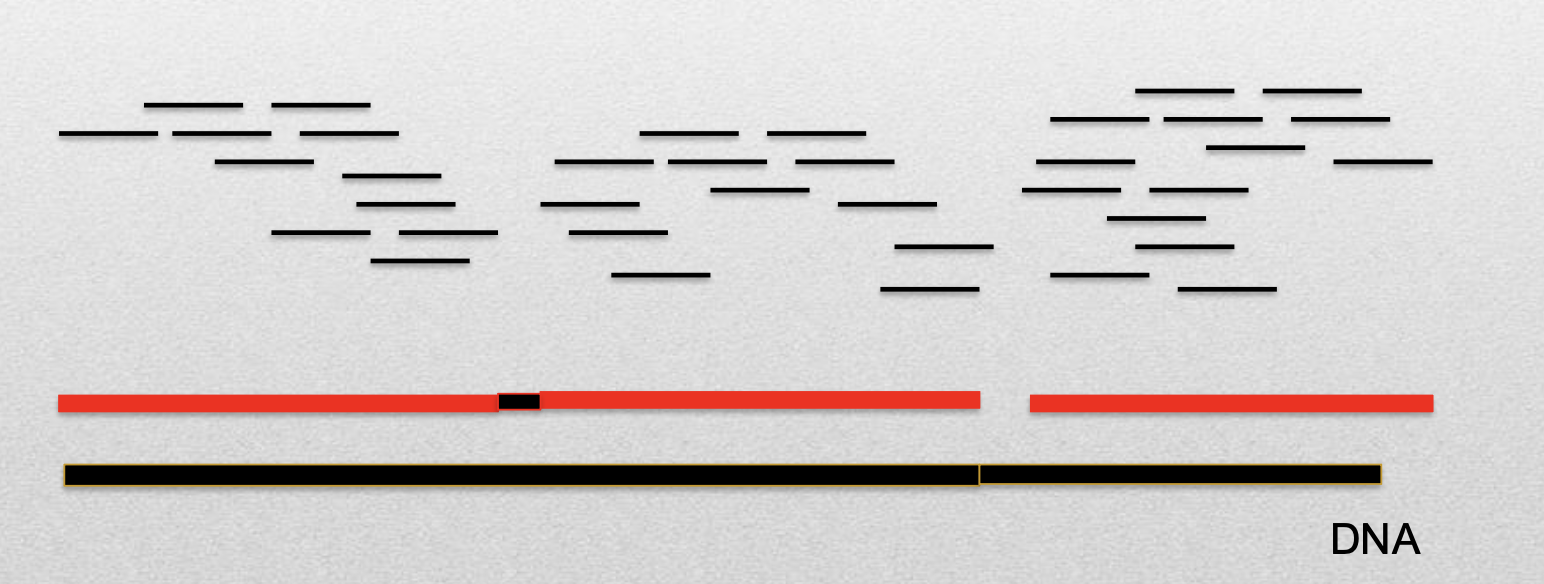
\includegraphics[width=0.7\textwidth]{images/assembly.png}
    \caption{4 fasi principali dell'assemblaggio di read}
    \label{fig:read-assembly}
\end{figure}

In particolare, la fase più rilevante per la definizione dei grafi è il contig assembly, 
che può essere affrontato con due metodi graph-based principali: \textbf{Overlap Layout Consensus (OLC)}, 
basato sugli overlap tra read, e \textbf{grafo di de Bruijn (dBG)}, basato sui k-mers.

\section*{Grafo di overlap}
Nel primo metodo, detto \textbf{Overlap Layout Consensus (OLC)}, si lavora direttamente sulle read, e l'assemblaggio avviene in
tre fasi:
\begin{itemize}
    \item Calcolo degli \textbf{overlap} tra le read
    \item costruzione dell’\textbf{Overlap Graph} per determinare il \textbf{layout}
    \item visita del grafo per ottenere il \textbf{consensus}
\end{itemize}

Questo approccio si basa sul problema \textbf{Shortest Common Superstring (SCS)} con:
\begin{itemize}
    \item \textbf{Input:} $r_1, r_2, \ldots, r_n$ stringhe su alfabeto $\Sigma$
    \item \textbf{Output:} stringa $G$ di minima lunghezza tale che ogni $r_i$ sia sottostringa di $G$.
\end{itemize}

L'idea è quindi di trovare una sequenza che contenga tutte le read, evitando di duplicare le porzioni sovrapposte. 
Quindi dati due read $r_i$ e $r_j$ si definisce l'\textbf{overlap} $ov(r_i, r_j)$ come il più lungo suffisso di $r_i$ 
che si ripete come prefisso di $r_j$ (o viceversa).

A partire dagli overlap è possibile definire il \textbf{grafo di overlap} $G = (V, A)$, dove:
\[
    V = \{r_1, r_2, \ldots, r_n\}
\]
e
\[
    A = \{(r_i, r_j) \mid r_i, r_j \in V, ov(r_i, r_j) \geq \tau\}
\]

dove $\tau$ rappresenta una soglia minima di overlap, introdotta per evitare di considerare sovrapposizioni 
troppo corte e quindi potenzialmente casuali. 

Un arco $(r_i,r_j)$ indica quindi che il read $r_j$ può seguire il read $r_i$ nell'assemblaggio.

A ogni arco $(r_i,r_j)$, inoltre, si associa un'etichetta:

\[
    ext(r_i, r_j)
\]

che rappresenta la parte di $r_j$ non contenuta nell'overlap con $r_i$, cioè la porzione che deve
essere aggiunta per estendere l'assemblaggio.

\begin{figure}[H]
    \centering
    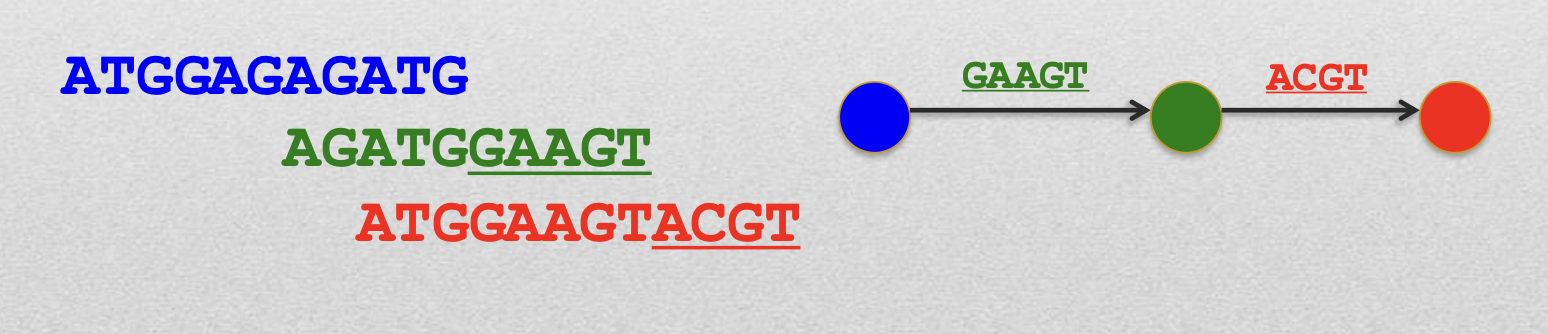
\includegraphics[width=0.7\textwidth]{images/overlap1.png}
    \caption{Grafo di overlap}
    \label{fig:overlap-graph}
\end{figure}

Se nel grafo considero un percorso:

\[
    \langle r_1, r_2, \ldots, r_p \rangle
\]

allora l'assembly lungo il percorso è:

\[
    r_1 \ ext(r_1,r_2) \ ext(r_2,r_3) \ \ldots \ ext(r_{p-1},r_p)
\]

Quindi l'assemblaggio non consiste nel concatenare interamente tutte le read,
ma nel partire dal primo read e aggiungere, per ogni arco attraversato, 
solo l'estensione del read successivo, evitando di duplicare le regioni sovrapposte.

In una versione ridotta del grafo, si possono eliminare gli archi transitivi, ottenendo:
\[
    A = \{(r_i, r_j) \mid r_i, r_j \in V, |ov(r_i, r_j)| \geq \tau, \ (r_i,r_j) \text{ non transitivo}\}
\]

Un arco è transitivo quando il collegamento diretto tra due read è già spiegato da un percorso 
che passa attraverso altri read; in tal caso l'arco diretto è ridondante e può essere rimosso.

In questo modello, poiché i vertici del grafo sono i read, 
l'obiettivo è trovare un ordine dei read che permetta di ricostruire una superstringa compatibile. 
Questo può essere visto come la ricerca di un cammino Hamiltoniano di peso massimo, 
dove il peso degli archi è dato dalla lunghezza degli overlap.

\section*{Grafo di De Bruijn}
Il secondo metodo per il contig assembly è basato sul \textbf{grafo di De Bruijn (dBG)}, che invece di lavorare direttamente sulle read,
le scompone in sottostringhe di lunghezza fissa $k$, dette \textbf{k-mers}.

Il contig assembly con dBG avviene in tre fasi:
\begin{itemize}
    \item Estrarre i k-mers dalle read
    \item costruzione del grafo di De Bruijn
    \item visita del grafo
\end{itemize}

Dato un alfabeto $\Sigma$, un k-mer di una stringa $r$ è un elemento di $\Sigma^k$, cioè una sottostringa di lunghezza $k$,
che occorre in $r$. Lo spettro di ordine $k$ di una stringa, o di una collezione di stringhe, 
è il multiset di tutti i k-mers presenti in essa. Si parla di multiset perché uno stesso k-mer
può comparire più volte, e ogni occorrenza è considerata distinta.

L'obiettivo del metodo è assemblare una sequenza di DNA attraverso la
determinazione del cammino Euleriano:
dato un grafo orientato $G = (V, A)$, per ogni vertice $v \in V$ si indicano con:
\begin{itemize}
    \item $IN(v)$: il numero di archi entranti in $v$
    \item $OUT(v)$: il numero di archi uscenti da $v$
\end{itemize}

Un \textbf{ciclo euleriano} è il ciclo che attraversa tutti gli archi del grafo una e una sola volta. Esiste quando il grafo è \textbf{bilanciato}, cioè:
\[
    \forall v \in V: IN(v) = OUT(v)
\]

Un \textbf{cammino euleriano} è un cammino che attraversa tutti gli archi una e una sola volta, senza dover
tornare al vertice iniziale. Esiste quando il grafo è \textbf{semi-bilanciato}, cioè: 
\begin{itemize}
    \item ha un nodo sorgente $v_s$ tale che $OUT(v_s) = IN(v_s) + 1$
    \item ha un nodo pozzo $v_t$ tale che $IN(v_t) = OUT(v_t) + 1$
    \item tutti gli altri nodi $v$ sono bilanciati, cioè $IN(v) = OUT(v)$
\end{itemize}

Esistono 3 definizioni di grafo di De Bruijn:
\begin{itemize}
    \item de Bruijn Graph classico
    \item Node-centric de Bruijn Graph
    \item Arc-centric de Bruijn Graph
\end{itemize}

\paragraph{de Bruijn Graph classico} 
Il grafo di De Bruijn classico di ordine $k$, definito su un alfabeto $\Sigma$ di $m$ simboli,
è un grafo orientato $G = (V, A)$, dove $V = \Sigma^k$, cioè i vertici sono tutte le possibili stringhe di lunghezza $k$ costruite sull'alfabeto $\Sigma$.

Esiste un arco orientato $(v_1, v_2)\in A$ se e solo il suffisso di $v_1$ di lunghezza $k-1$ è uguale al prefisso di $v_2$ di lunghezza $k-1$:
\[
    (v_1, v_2) \in A \iff suff_{k-1}(v_1) = pref_{k-1}(v_2)
\]
Ogni arco $(v_1, v_2)$ rappresenta quindi la possibilità di concatenare $v_1$ e $v_2$ sovrapponendo i loro $k-1$ simboli.
L'arco è etichettato dalla stringa ottenuta aggiungendo a $v_1$ l'ultimo simbolo di $v_2$.
Il grafo ottenuto è un grafo bilanciato.
\begin{figure}[H]
    \centering
    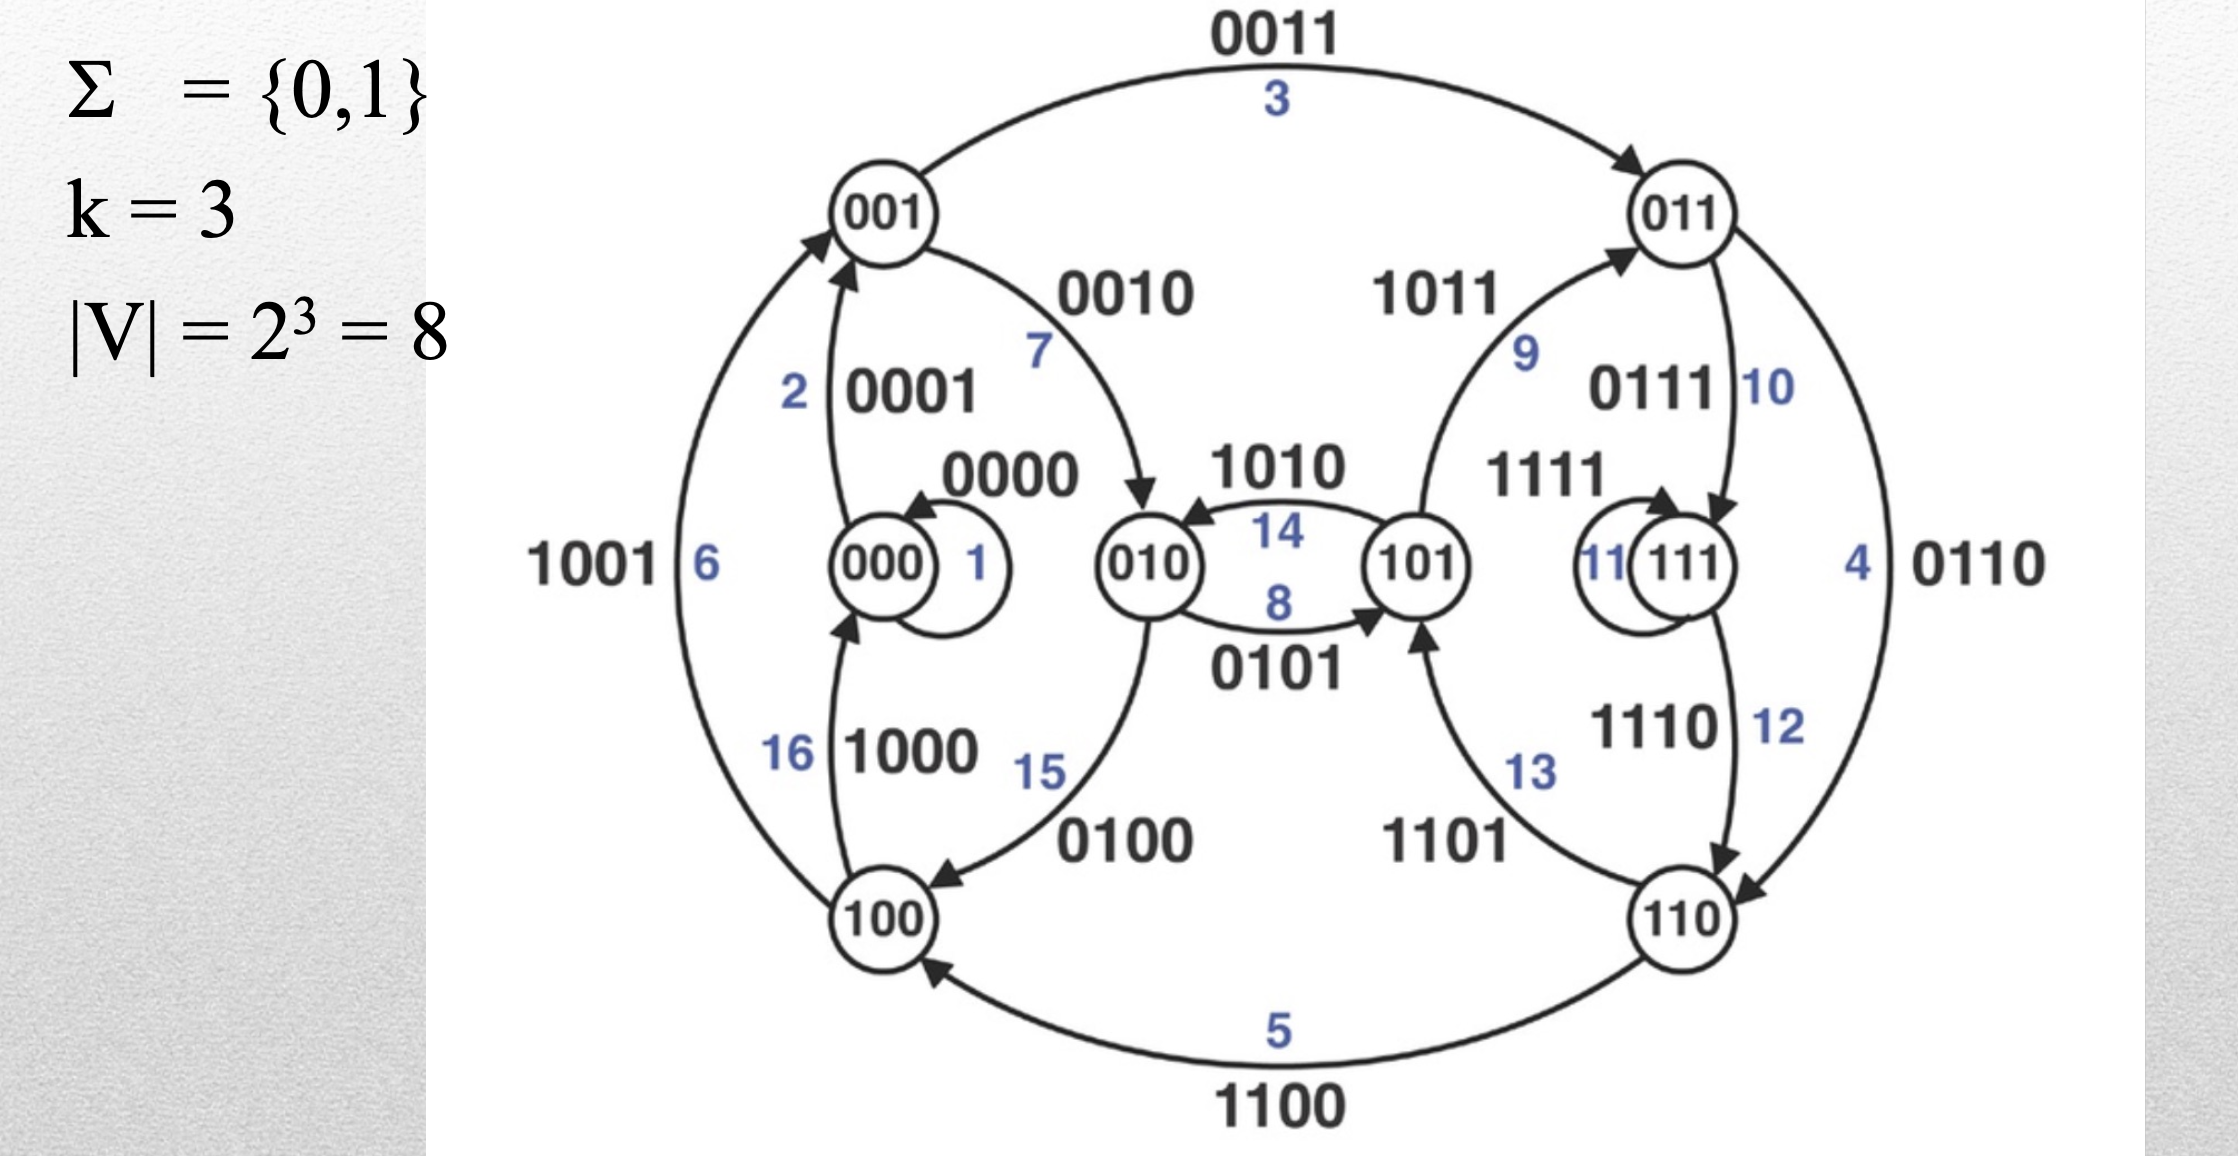
\includegraphics[width=0.7\textwidth]{images/dbgClassico.png}
    \caption{Grafo di De Bruijn classico}
    \label{fig:dbg-classico}
\end{figure}

\paragraph{Node-centric de Bruijn Graph}
Dato un insieme di read $\{r_1, r_2, \ldots, r_n\}$, il node-centric de Bruijn Graph di ordine $k$
è un grafo orientato $G = (V, A)$, dove:
\[
    V = \{\text{k-mer distinti nello spettro di ordine } k \text{ delle read}\}
\]
Quindi i nodi nel grafo sono i k-mers estratti dalle read.
Esiste un arco orientato $(v_1, v_2)\in A$ se e solo il suffisso di $v_1$ di lunghezza $k-1$ è uguale al prefisso di $v_2$ di lunghezza $k-1$:
\[
    (v_1, v_2) \in A \iff suff_{k-1}(v_1) = pref_{k-1}(v_2)
\]
Ogni arco $(v_1, v_2)$ è etichettato con l'ultimo simbolo di $v_2$.
Se considero un cammino $ \langle v_1, v_2, \ldots, v_p \rangle$ l'assembly si ottiene scrivendo 
il primo k-mer $v_1$ e poi aggiungendo progressivamente l’ultimo simbolo dei vertici successivi:
\[
    v_1 \ last(v_2) \ last(v_3) \ \ldots \ last(v_p)
\]
\begin{figure}[H]
    \centering
    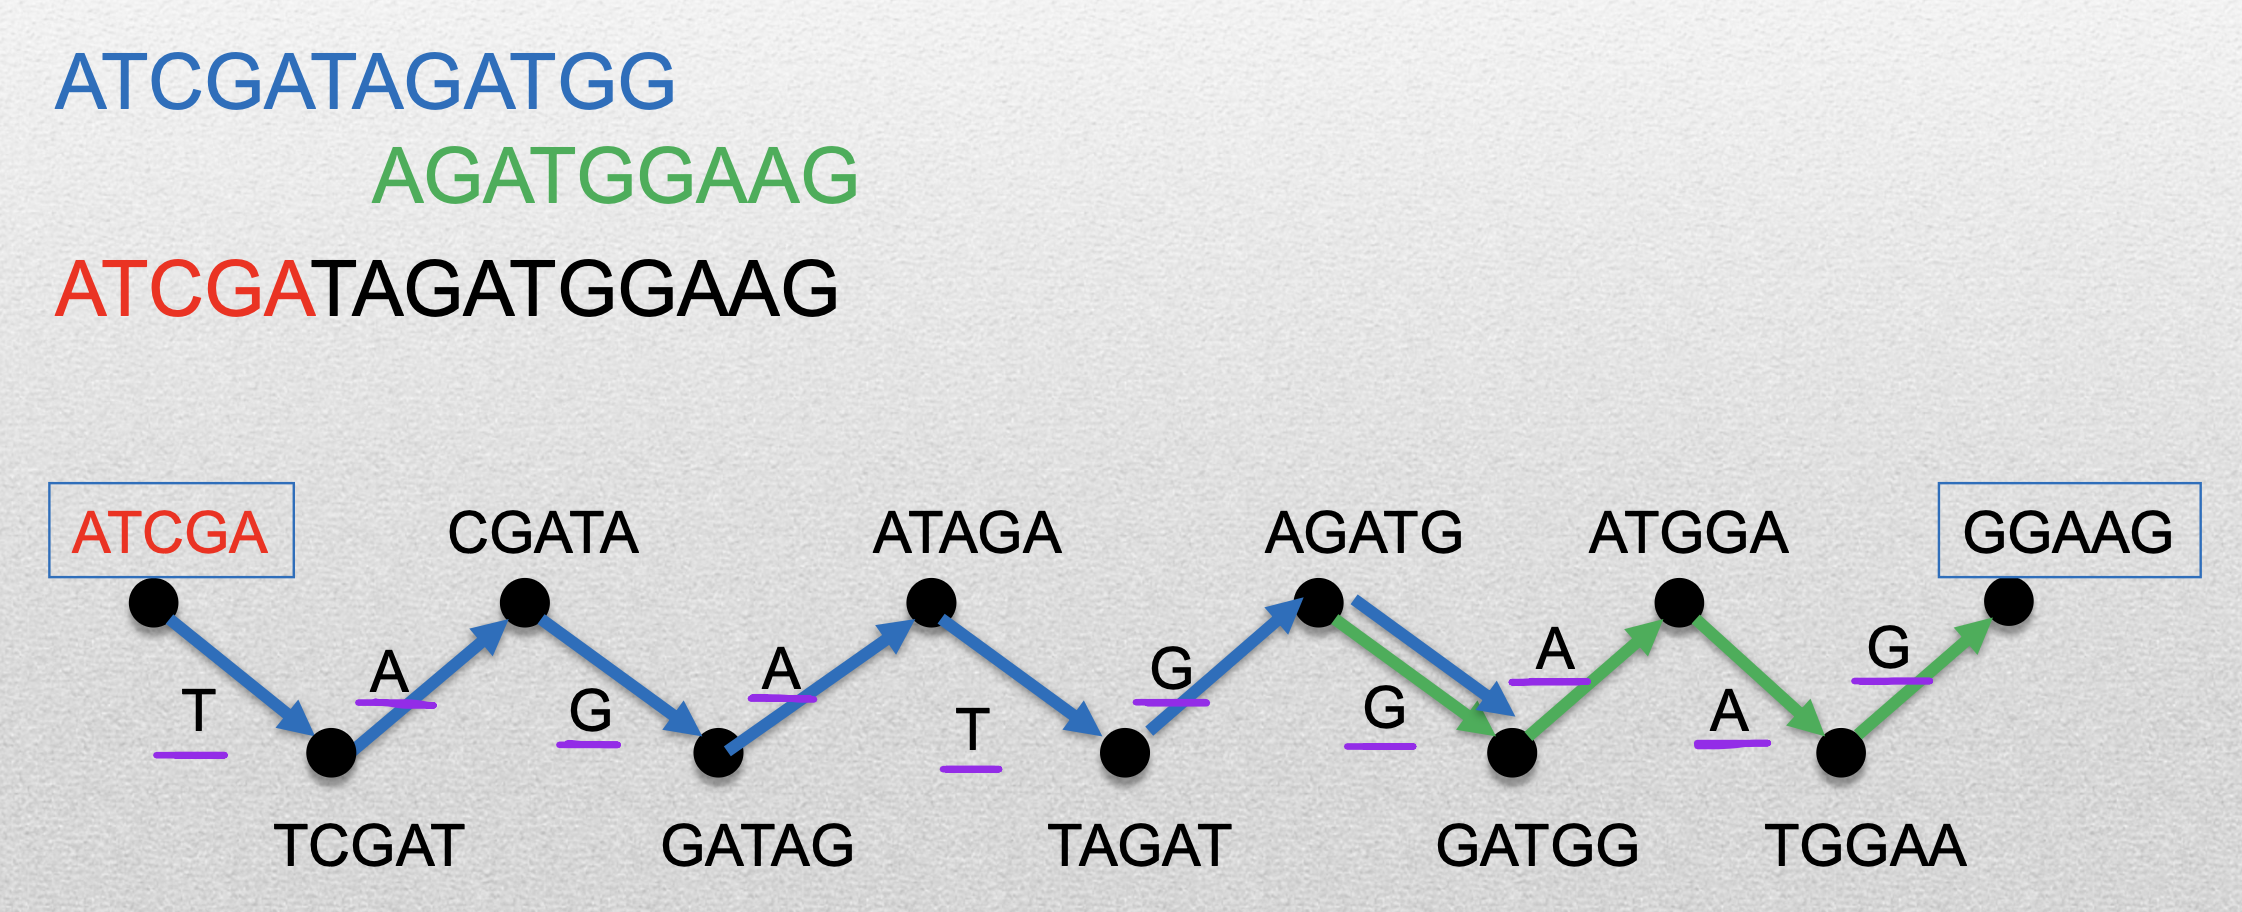
\includegraphics[width=0.8\textwidth]{images/dbgNode.png}
    \caption{Grafo di De Bruijn node-centric di ordine 5}
    \label{fig:dbg-node-centric}
\end{figure}

\paragraph{Arc-centric de Bruijn Graph}
Dato un insieme di read $\{r_1, r_2, \ldots, r_n\}$,
l'arc-centric de Bruijn Graph di ordine $k$ è un grafo orientato $G = (V, A)$, dove:
\[
    V = \{\text{(k-1)-mer distinti nello spettro di ordine (k-1) delle read}\}
\]
Quindi, in questa definizione, i nodi sono i (k-1)-mers.
L'arco orientato $(v_1, v_2) \in A$ esiste se e solo se 
\[
    suff_{k-2}(v_1) = pref_{k-2}(v_2)
\]
e se l'assembly ottenuto concatenando $v_1$ e l'ultimo simbolo 
di $v_2$ è un k-mer presente nello spettro di ordine k delle read.

In modo equivalente, per ogni k-mer osservato nelle read si costruisce
un arco dal prefisso di lunghezza $k-1$ al suo suffisso di lunghezza $k-1$.
Ogni arco è etichettato con l'ultimo simbolo di $v_2$.

Essendo che ogni arco rappresenta un k-mer osservato nelle read.
Per questo motivo, assemblare la sequenza significa trovare un cammino euleriano,
cioè un cammino che attraversa tutti gli archi una e una sola volta.

Se il grafo deriva da una sequenza lineare, allora è semi-bilanciato: esiste
un nodo sorgente, che corrisponde all'inizio della sequenza, e un nodo pozzo,
che corrisponde alla fine della sequenza.

Se considero un cammino euleriano
\[
    \langle v_1, v_2, \ldots, v_p \rangle
\]
l'assembly si ottiene scrivendo il primo $(k-1)$-mer $v_1$ e poi aggiungendo
progressivamente l'ultimo simbolo dei vertici successivi:
\[
    v_1 \ last(v_2) \ last(v_3) \ \ldots \ last(v_p)
\]

\begin{figure}[H]
    \centering
    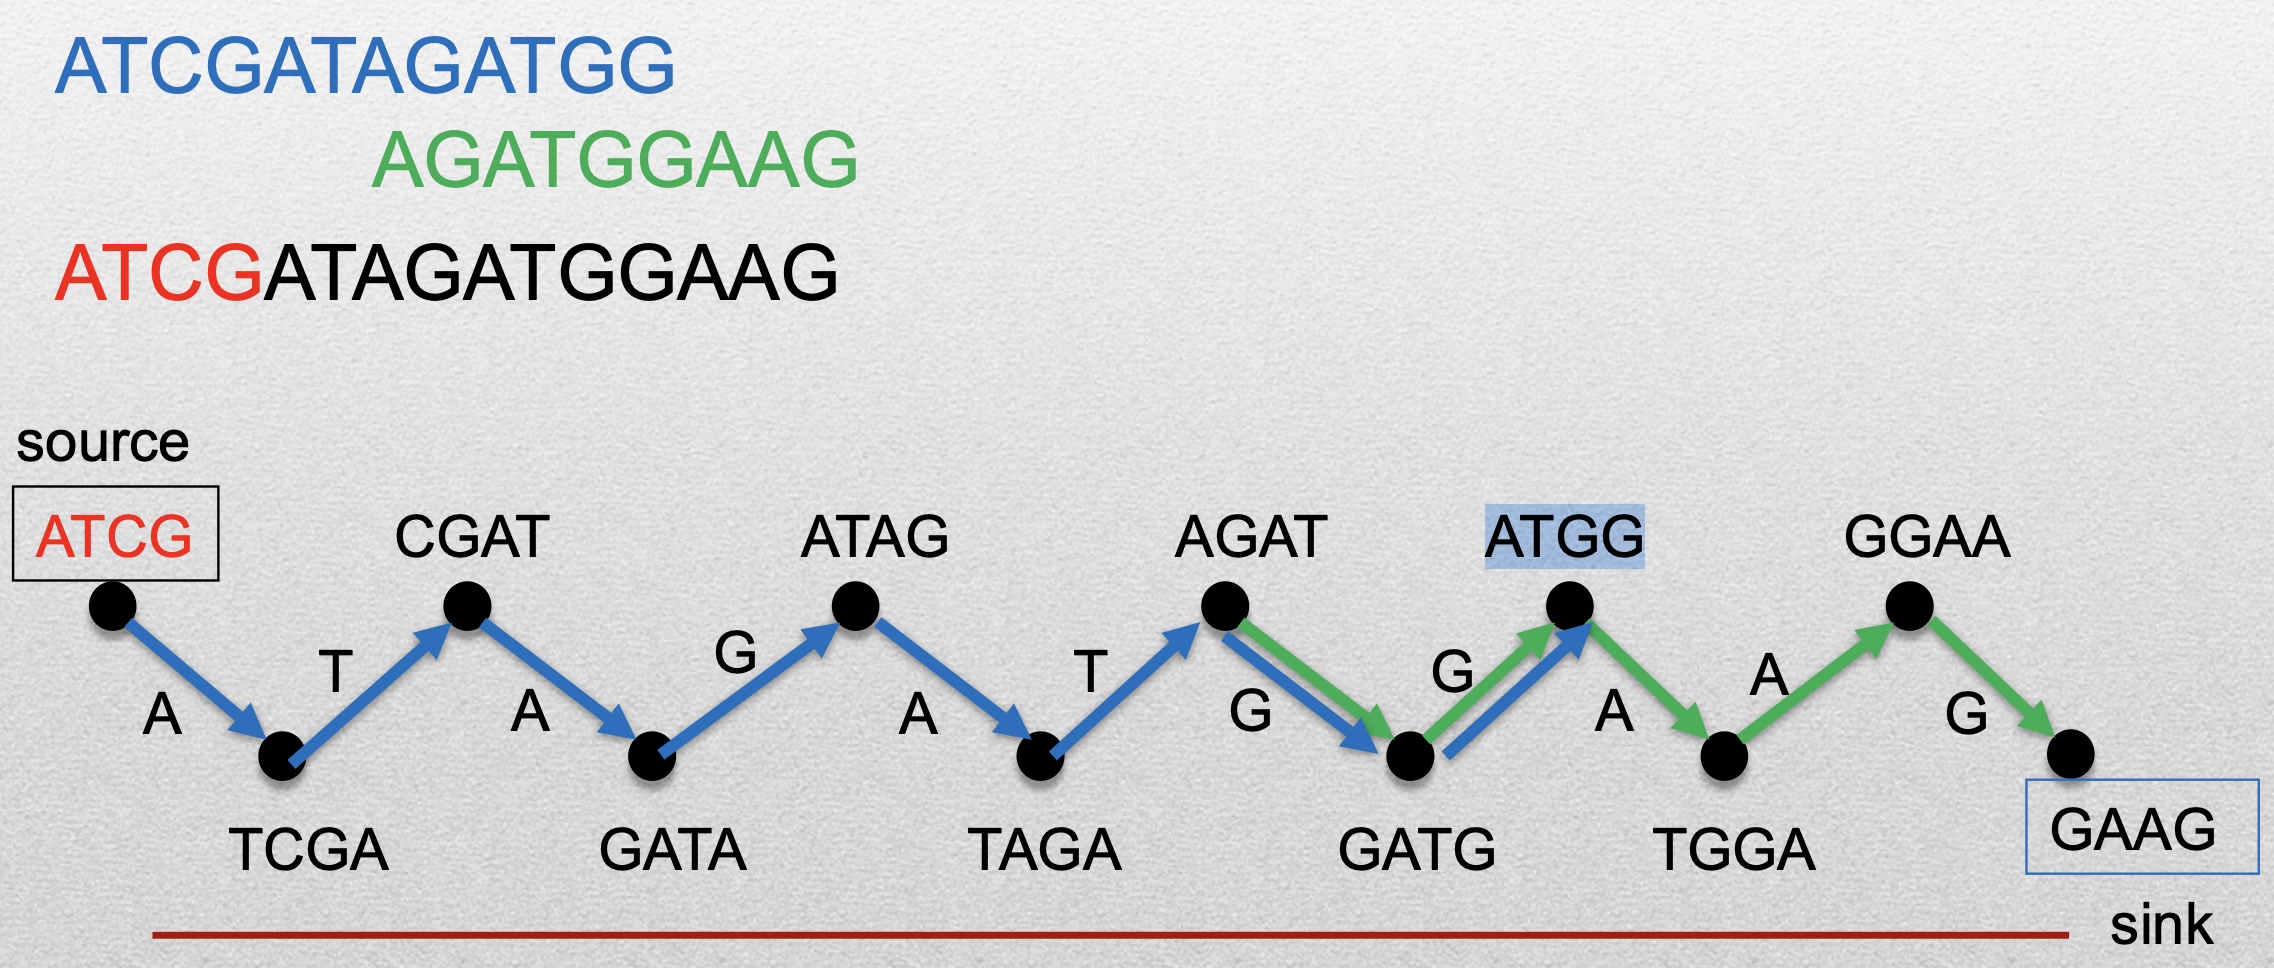
\includegraphics[width=0.8\textwidth]{images/dbgArc.png}
    \caption{Grafo di De Bruijn arc-centric di ordine 5}
    \label{fig:dbg-arc-centric}
\end{figure}

\paragraph{Problemi nella costruzione del dBG}

Nella pratica, il grafo di De Bruijn può presentare alcune strutture problematiche.
I \textbf{loop} sono archi che partono e arrivano nello stesso nodo. Si formano
quando un k-mer collega un $(k-1)$-mer con sé stesso.
Le \textbf{ripetizioni}, invece, sono regioni ripetute della sequenza che possono
rendere ambiguo il cammino euleriano, producendo più assembly compatibili
con lo stesso grafo.
Inoltre, gli errori di sequenziamento possono introdurre k-mers errati, che generano
strutture problematiche nel grafo. Le più comuni sono:

\begin{itemize}
    \item \textbf{tips}: ramificazioni corte senza prosecuzione, spesso dovute a errori
    nelle estremità delle read;
    \item \textbf{bubbles}: cammini alternativi tra due stessi nodi, spesso causati da
    errori di sequenziamento o varianti molto simili.
\end{itemize}

La scelta del valore di $k$ è quindi importante: un valore troppo piccolo può aumentare
le ambiguità dovute alle ripetizioni, mentre un valore troppo grande può frammentare
il grafo, soprattutto in presenza di errori o bassa copertura.
